\documentclass{article}

\usepackage{arxiv}

\usepackage[utf8]{inputenc} % allow utf-8 input
\usepackage[T1]{fontenc}    % use 8-bit T1 fonts
\usepackage{lmodern}        % https://github.com/rstudio/rticles/issues/343
\usepackage{hyperref}       % hyperlinks
\usepackage{url}            % simple URL typesetting
\usepackage{booktabs}       % professional-quality tables
\usepackage{amsfonts}       % blackboard math symbols
\usepackage{nicefrac}       % compact symbols for 1/2, etc.
\usepackage{microtype}      % microtypography
\usepackage{lipsum}
\usepackage{graphicx}

\title{A template for the \emph{arxiv} style}

\author{
    H.Sherry Zhang
   \\
    Department of Econometrics and Business Statistics \\
    Monash University \\
  Melbourne, Australia \\
  \texttt{\href{mailto:huize.zhang@monash.edu}{\nolinkurl{huize.zhang@monash.edu}}} \\
   \And
    Dianne Cook
   \\
    Department of Econometrics and Business Statistics \\
    Monash University \\
  Melbourne, Australia \\
  \texttt{\href{mailto:dicook@monash.edu}{\nolinkurl{dicook@monash.edu}}} \\
   \And
    Ursula Laa
   \\
    Institute of Statistics \\
    University of Natural Resources and Life Sciences \\
  Vienna, Austria \\
  \texttt{\href{mailto:ursula.laa@boku.ac.at}{\nolinkurl{ursula.laa@boku.ac.at}}} \\
   \And
    Nicolas Langrené
   \\
    34 Village Street, Docklands VIC 3008 Australia \\
    CSIRO Data61 \\
  Melbourne, Australia \\
  \texttt{\href{mailto:nicolas.langrene@csiro.au}{\nolinkurl{nicolas.langrene@csiro.au}}} \\
   \And
    Patricia Menéndez
   \\
    Department of Econometrics and Business Statistics \\
    Monash University \\
  Melbourne, Australia \\
  \texttt{\href{mailto:patricia.menendez@monash.edu}{\nolinkurl{patricia.menendez@monash.edu}}} \\
  }

\usepackage{color}
\usepackage{fancyvrb}
\newcommand{\VerbBar}{|}
\newcommand{\VERB}{\Verb[commandchars=\\\{\}]}
\DefineVerbatimEnvironment{Highlighting}{Verbatim}{commandchars=\\\{\}}
% Add ',fontsize=\small' for more characters per line
\usepackage{framed}
\definecolor{shadecolor}{RGB}{248,248,248}
\newenvironment{Shaded}{\begin{snugshade}}{\end{snugshade}}
\newcommand{\AlertTok}[1]{\textcolor[rgb]{0.94,0.16,0.16}{#1}}
\newcommand{\AnnotationTok}[1]{\textcolor[rgb]{0.56,0.35,0.01}{\textbf{\textit{#1}}}}
\newcommand{\AttributeTok}[1]{\textcolor[rgb]{0.77,0.63,0.00}{#1}}
\newcommand{\BaseNTok}[1]{\textcolor[rgb]{0.00,0.00,0.81}{#1}}
\newcommand{\BuiltInTok}[1]{#1}
\newcommand{\CharTok}[1]{\textcolor[rgb]{0.31,0.60,0.02}{#1}}
\newcommand{\CommentTok}[1]{\textcolor[rgb]{0.56,0.35,0.01}{\textit{#1}}}
\newcommand{\CommentVarTok}[1]{\textcolor[rgb]{0.56,0.35,0.01}{\textbf{\textit{#1}}}}
\newcommand{\ConstantTok}[1]{\textcolor[rgb]{0.00,0.00,0.00}{#1}}
\newcommand{\ControlFlowTok}[1]{\textcolor[rgb]{0.13,0.29,0.53}{\textbf{#1}}}
\newcommand{\DataTypeTok}[1]{\textcolor[rgb]{0.13,0.29,0.53}{#1}}
\newcommand{\DecValTok}[1]{\textcolor[rgb]{0.00,0.00,0.81}{#1}}
\newcommand{\DocumentationTok}[1]{\textcolor[rgb]{0.56,0.35,0.01}{\textbf{\textit{#1}}}}
\newcommand{\ErrorTok}[1]{\textcolor[rgb]{0.64,0.00,0.00}{\textbf{#1}}}
\newcommand{\ExtensionTok}[1]{#1}
\newcommand{\FloatTok}[1]{\textcolor[rgb]{0.00,0.00,0.81}{#1}}
\newcommand{\FunctionTok}[1]{\textcolor[rgb]{0.00,0.00,0.00}{#1}}
\newcommand{\ImportTok}[1]{#1}
\newcommand{\InformationTok}[1]{\textcolor[rgb]{0.56,0.35,0.01}{\textbf{\textit{#1}}}}
\newcommand{\KeywordTok}[1]{\textcolor[rgb]{0.13,0.29,0.53}{\textbf{#1}}}
\newcommand{\NormalTok}[1]{#1}
\newcommand{\OperatorTok}[1]{\textcolor[rgb]{0.81,0.36,0.00}{\textbf{#1}}}
\newcommand{\OtherTok}[1]{\textcolor[rgb]{0.56,0.35,0.01}{#1}}
\newcommand{\PreprocessorTok}[1]{\textcolor[rgb]{0.56,0.35,0.01}{\textit{#1}}}
\newcommand{\RegionMarkerTok}[1]{#1}
\newcommand{\SpecialCharTok}[1]{\textcolor[rgb]{0.00,0.00,0.00}{#1}}
\newcommand{\SpecialStringTok}[1]{\textcolor[rgb]{0.31,0.60,0.02}{#1}}
\newcommand{\StringTok}[1]{\textcolor[rgb]{0.31,0.60,0.02}{#1}}
\newcommand{\VariableTok}[1]{\textcolor[rgb]{0.00,0.00,0.00}{#1}}
\newcommand{\VerbatimStringTok}[1]{\textcolor[rgb]{0.31,0.60,0.02}{#1}}
\newcommand{\WarningTok}[1]{\textcolor[rgb]{0.56,0.35,0.01}{\textbf{\textit{#1}}}}

% Pandoc citation processing
\newlength{\csllabelwidth}
\setlength{\csllabelwidth}{3em}
\newlength{\cslhangindent}
\setlength{\cslhangindent}{1.5em}
% for Pandoc 2.8 to 2.10.1
\newenvironment{cslreferences}%
  {}%
  {\par}
% For Pandoc 2.11+
\newenvironment{CSLReferences}[2] % #1 hanging-ident, #2 entry spacing
 {% don't indent paragraphs
  \setlength{\parindent}{0pt}
  % turn on hanging indent if param 1 is 1
  \ifodd #1 \everypar{\setlength{\hangindent}{\cslhangindent}}\ignorespaces\fi
  % set entry spacing
  \ifnum #2 > 0
  \setlength{\parskip}{#2\baselineskip}
  \fi
 }%
 {}
\usepackage{calc} % for calculating minipage widths
\newcommand{\CSLBlock}[1]{#1\hfill\break}
\newcommand{\CSLLeftMargin}[1]{\parbox[t]{\csllabelwidth}{#1}}
\newcommand{\CSLRightInline}[1]{\parbox[t]{\linewidth - \csllabelwidth}{#1}\break}
\newcommand{\CSLIndent}[1]{\hspace{\cslhangindent}#1}



\begin{document}
\maketitle

\def\tightlist{}


\begin{abstract}
Enter the text of your abstract here.
\end{abstract}

\keywords{
    blah
   \and
    blee
   \and
    bloo
   \and
    these are optional and can be removed
  }

\newpage

\hypertarget{introduction}{%
\section{Introduction}\label{introduction}}

Spatio-temporal data record changes of variables in spatially separated
regions across time. In this article, we consider spatio-temporal vector
data, which are recorded in a fixed interval and are point based,
characterised by longitude and latitude, in the spatial aspect. Examples
of this type of data include the house price of a city or county,
climate measures from weather stations in a country, and river level
data from electronic gauges.

Analysing this type of data requires less considerations on the
geographical geometry type and map projection but more on how measures
in these fixed locations changes across the time domain and whether
these changes are related for adjacent locations. For example, when
nearby areas show patterns that are regular enough, visualising
spatio-temporal data can 1) discover regional time series features,
i.e.~trend and seasonality, 2) find the Waldo sites from the crowd, and
3) see how correlation of nearby sites changes across time.

The main difficulty in visualising this type of data is to show
information in both space and time dimension with the proper level of
details without information overflow. This would sometimes require
aggregating the time dimension into the proper level or slicing the data
into a reasonable number of subset for display. In this sense, a data
structure that regulates the manipulation spatio-temporal data will
benefit the analysis workflow. While many implementations focus on
manipulating and visualising pure spatial or temporal data, there are
not sufficient tools to deal with spatio-temporal data. The purpose of
this paper is to introduce a spatio-temporal vector data structure for
data analysis in R.

The rest of the paper will be divided as follows: Section 2 reviews the
existing data structure for spatio, temporal, and spatio-temporal data.
Section 3 presents a new data structure for spatio-temporal data:
cubble. Then the paper introduces the workflow of data manipulation and
visualisation with the cubble structure in Section 4. Section 5 gives
some examples on how common spatial and temporal manipulations are
performed with cubble and how static and interactive visualisation help
to understand climate and {[}\ldots{]} data.

\hypertarget{existing-data-structure-for-spatio-and-temporal-data}{%
\section{Existing data structure for spatio and temporal
data}\label{existing-data-structure-for-spatio-and-temporal-data}}

Below we review some structure for spatial, temporal, and
spatio-temporal data.

Many spatial and spatio-temporal data structures have been developed by
the R-spatial team for both raster and vector spatial data. For vector
spatial data, which is the focus of this paper, \texttt{sf} (E. J.
Pebesma 2018) represents spatial vector information with simple
features: points, lines, polygons and their multiples. Various
\texttt{st\_} function are designed to manipulate these features based
on their geometric relationships. For spatio-temporal data,
\texttt{stars} (E. Pebesma 2021) can represent both raster and vector
data using multi-dimensional array. However, the underlying array
structure can be difficult to operate for data analysts who are more
familiar with a flat 2D data frame structure used by the tidyverse
ecosystem.

In the temporal aspect, the \texttt{tsibble} (Wang, Cook, and Hyndman
2020) structure and its tidyverts ecosystem have provided a {[}\ldots{}
{]} workflow to work with temporal data. In a tsibble structure,
temporal data is characterised by \texttt{index} and \texttt{key} where
\texttt{index} is the temporal identifier and \texttt{key} is the
identifier for multiple series, which could be used as a spatio
identifier. However, a tsibble object, by construction, always requires
the \texttt{index} in its structure. This makes it less appealing for
spatio-temporal data since the output of calculated spatio-specific
variables (i.e.~features of each series) don't have the time dimension.
Analysts will either need to have an additional step to join this output
to the original tsibble or operate with variables stored in two separate
objects. In addition, the long form structure of a tsibble object means
spatio variables (i.e.~longitude, latitude, and features of each series
if joined back to the tsibble) of each spatio identifier will be
repetitively recorded at each timestamp. This repetition is unnecessary
and would inflate the object size for long series.

\textcolor{red}{Under the third tidy data principle [@tidydata], these are two type of observational unit and should form different tables. An example (Table 8) is also given to demonstrate the billboard dataset where there are song variables and rank variables that changes each week. The other has mentioned the lack of tool to work directly with relational data and analysis will usually need to merge the dataset into one table, which could causes errors. These days more implementations have looked at relational data structure and in R, several good examples include, `tidygraph`[@tidygraph] for graph manipulation, `dm` [@dm] for relational data model. In the domain of spatio-temporal data, @spacetime has considered four types of spatio-temporal layout. `Spatstat` [@Spatstat] an implementation of point pattern.  }

\newpage

\hypertarget{a-new-data-structure-for-spatio-temporal-data}{%
\section{A new data structure for spatio-temporal
data}\label{a-new-data-structure-for-spatio-temporal-data}}

Spatio-temporal data don't usually come to the analysts as a whole
piece. A way to look at these data is to divide it into spatial and
temporal dimension with an ID that links between the two. The first row
in Figure \ref{fig:cubble-diagram} illustrates this representation where
in the spatial dimension, the data is characterised by \texttt{id},
\texttt{lat}, \texttt{long}. \(V_s\) in the last column represents all
the other site-wise variables, for example, elevation and full name etc.
The temporal dimension, on the other hand, can be characterised by
\texttt{id} and \texttt{t} with \(V_t\) representing all the time-wise
variables. In climate data, this could include precipitation, maximum or
minimum temperature, and wind speed etc.

\begin{figure}

{\centering 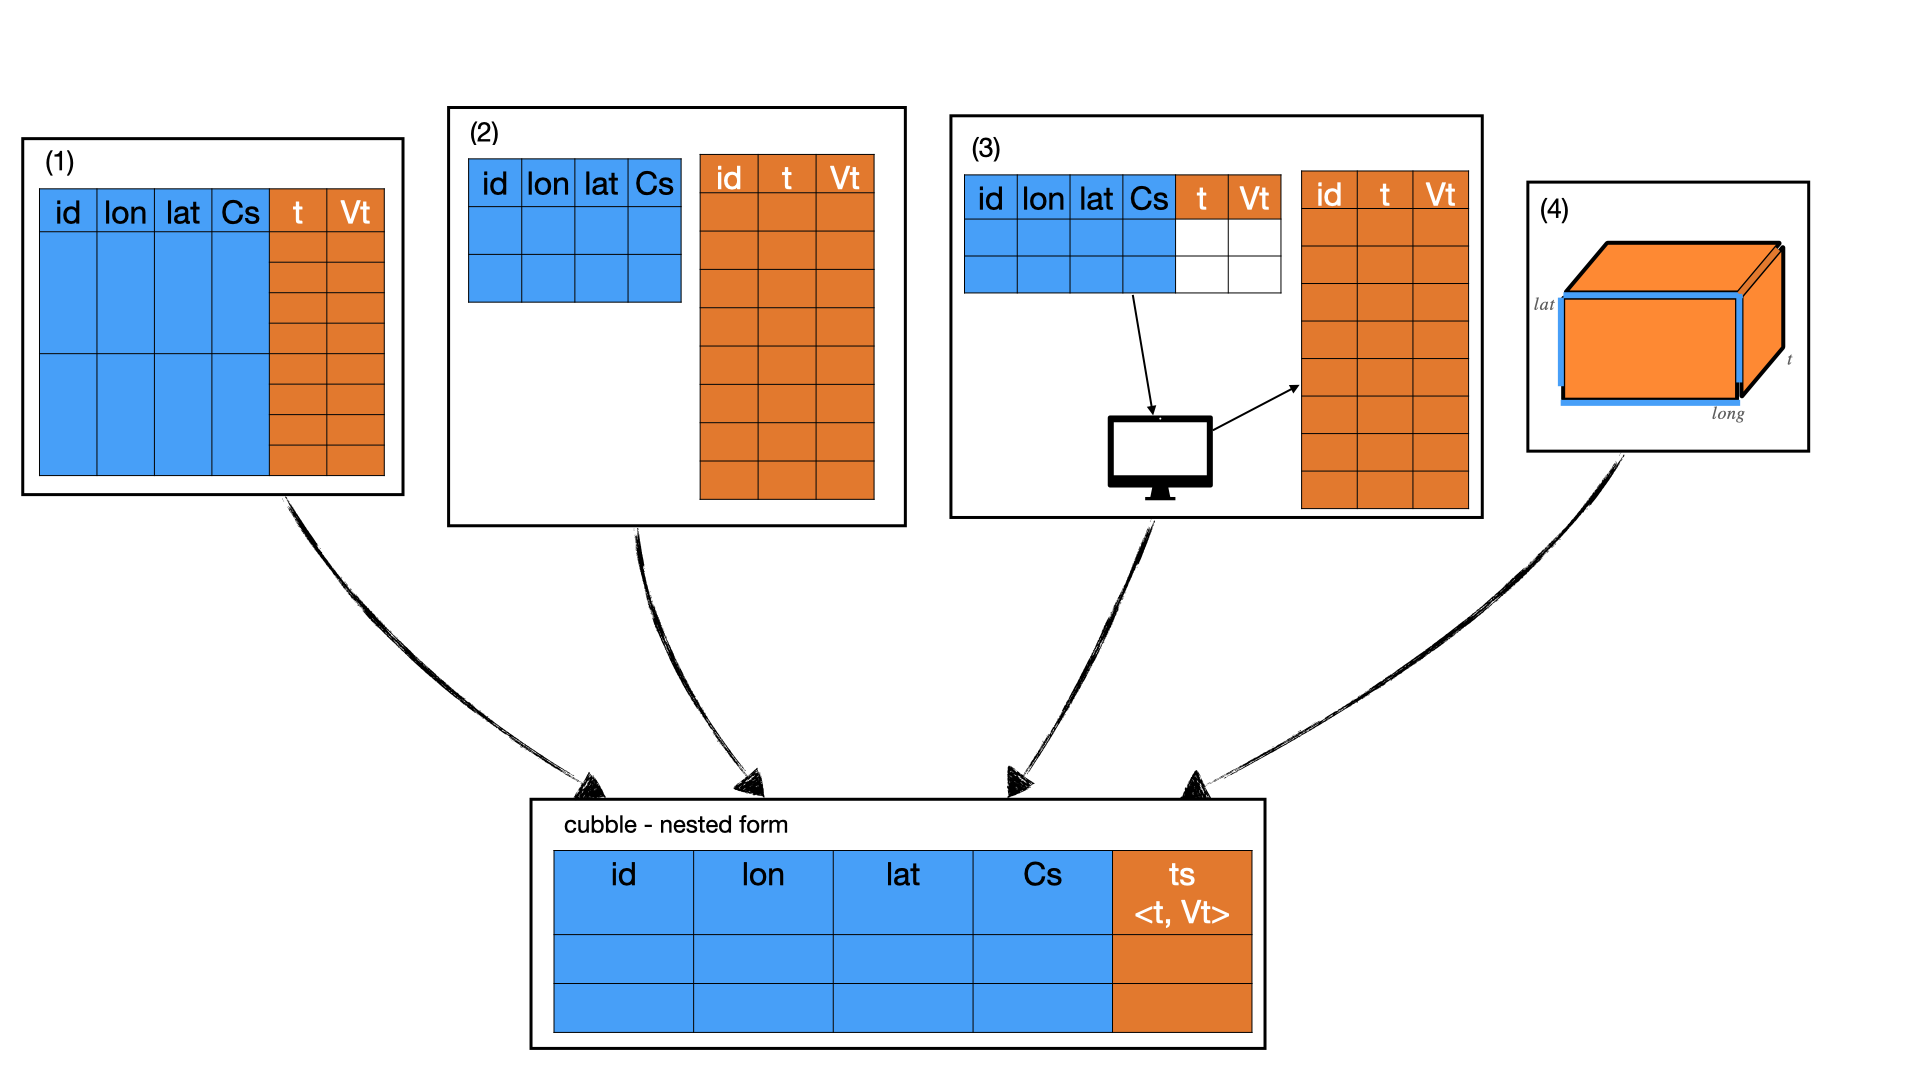
\includegraphics[width=1\linewidth,height=0.4\textheight]{/Users/sherryzhang/Documents/research/paper-cubble/figures/input-formats/input-formats.001} 

}

\caption{Cubble diagram}\label{fig:cubble-diagram}
\end{figure}

To work with spatio-temporal data, analysts can choose to either work
separately on each dimension or join the two sets together, however,
each approach has its own problem: While is is natural to work
separately on each sheet (since spatial and temporal operations usually
don't overlap), analysts will need to manually keep the other data frame
up to date. For example, the following pseudo code illustrates the
scenario where once the spatial dataset is filtered for those within
Victoria, the temporal dataset needs to be manually updated to reflect
this spatial filter.

\begin{Shaded}
\begin{Highlighting}[]
\NormalTok{spatial\_new }\OtherTok{\textless{}{-}}\NormalTok{ spatial }\SpecialCharTok{\%\textgreater{}\%} \FunctionTok{filter}\NormalTok{(SITES\_IN\_VICTORIA)}
\NormalTok{temporal\_new }\OtherTok{\textless{}{-}}\NormalTok{ temporal }\SpecialCharTok{\%\textgreater{}\%} \FunctionTok{filter}\NormalTok{(id }\SpecialCharTok{\%in\%}\NormalTok{ spatial\_new}\SpecialCharTok{$}\NormalTok{id)}
\end{Highlighting}
\end{Shaded}

If analysts choose to join the spatial and temporal data together, the
joined dataset could be too large since each spatial variable will be
repeated at each time stamp for each site. Also, recordings of the site
ID from different data sources can be slightly different from each
other, causing a painful checking and cleaning of site IDs before the
join.

A cubble, in essence, wires both dimensions in the spatio-temporal data
into one object while provide two forms for manipulation the spatial and
temporal dimension separately.

When manipulating the spatial dimension it uses a nest form that:

\begin{itemize}
\tightlist
\item
  defines each group in a row,
\item
  displays the group-related variables in columns, and
\item
  nests all the time-related variables into a column called \texttt{ts}.
\end{itemize}

When manipulating the temporal dimension, it uses the long form that:

\begin{itemize}
\tightlist
\item
  each combination of group and timestamp occupies a row
\item
  time-related variables are displayed, and
\item
  group-related variables are not explicitly displayed but can be
  accessed through the \texttt{meta} attribute.
\end{itemize}

\newpage

\hypertarget{create-a-cubble}{%
\section{Create a cubble}\label{create-a-cubble}}

The creation of a cubble requires the site identifier (\texttt{key}), as
well as the spatial (\texttt{coords}) and temporal (\texttt{index})
identifier. \texttt{climate\_flat} is already a tibble and it uses
\texttt{id} to identify each station, \texttt{date} as the time
identifier, and \texttt{c(long,\ lat)} as the spatial identifier. To
create a cubble for this data, use:

\begin{Shaded}
\begin{Highlighting}[]
\NormalTok{climate\_flat }\SpecialCharTok{\%\textgreater{}\%} \FunctionTok{as\_cubble}\NormalTok{(}\AttributeTok{key =}\NormalTok{ id, }\AttributeTok{index =}\NormalTok{ date, }\AttributeTok{coords =} \FunctionTok{c}\NormalTok{(long, lat))}
\end{Highlighting}
\end{Shaded}

\begin{verbatim}
## # Cubble: id-wise: nested form
## # Key:    id [5]
## # Leaves: date [date], prcp [dbl], tmax [dbl], tmin [dbl]
##   id            lat  long  elev name           wmo_id ts                
##   <chr>       <dbl> <dbl> <dbl> <chr>           <dbl> <list>            
## 1 ASN00009021 -31.9  116.  15.4 perth airport   94610 <tibble [366 x 4]>
## 2 ASN00010311 -31.9  117. 179   york            94623 <tibble [366 x 4]>
## 3 ASN00010614 -32.9  117. 338   narrogin        94627 <tibble [366 x 4]>
## 4 ASN00014015 -12.4  131.  30.4 darwin airport  94120 <tibble [366 x 4]>
## 5 ASN00015131 -17.6  134. 220   elliott         94236 <tibble [366 x 4]>
\end{verbatim}

Most of the time, spatio-temporal data doesn't come into this form and
analysts need to query the climate variables based on station metadata.
\textcolor{red}{This is also a problem illustrated in Section 3.5 in @tidydata. Here we provide a structured way to query this data based on the row-wise operator and nested list.}
For this type of task, one can structure a metadata into a tibble and
use row-wise operator to query the climate variables into a nested list.
As an example here we demonstrate the workflow to find the 5 closest
stations to Melbourne. We first create a station data frame with the 5
target stations.

\begin{verbatim}
## # A tibble: 5 x 8
##   id            lat  long  elev name                 wmo_id  dist city     
##   <chr>       <dbl> <dbl> <dbl> <chr>                 <dbl> <dbl> <chr>    
## 1 ASN00086038 -37.7  145.  78.4 essendon airport      95866  10.8 melbourne
## 2 ASN00086282 -37.7  145. 113.  melbourne airport     94866  20.1 melbourne
## 3 ASN00086077 -38.0  145.  12.1 moorabbin airport     94870  21.9 melbourne
## 4 ASN00088162 -37.4  145. 528.  wallan (kilmore gap)  94860  48.1 melbourne
## 5 ASN00087113 -38.0  144.  10.6 avalon airport        94854  48.8 melbourne
\end{verbatim}

We can query the climate information into a nested list named
\texttt{ts} for each station with the \texttt{rowwise()} operator. To
create a cubble, supply the same identifiers as with the first example.

\begin{Shaded}
\begin{Highlighting}[]
\NormalTok{sydmel\_climate }\OtherTok{\textless{}{-}}\NormalTok{ stations }\SpecialCharTok{\%\textgreater{}\%} 
  \FunctionTok{rowwise}\NormalTok{() }\SpecialCharTok{\%\textgreater{}\%} 
  \FunctionTok{mutate}\NormalTok{(}\AttributeTok{ts =} \FunctionTok{list}\NormalTok{(}\FunctionTok{meteo\_pull\_monitors}\NormalTok{(id, }
                                       \AttributeTok{date\_min =} \StringTok{"2020{-}01{-}01"}\NormalTok{, }
                                       \AttributeTok{date\_max =} \StringTok{"2020{-}12{-}31"}\NormalTok{,}
                                       \AttributeTok{var =} \FunctionTok{c}\NormalTok{(}\StringTok{"PRCP"}\NormalTok{, }\StringTok{"TMAX"}\NormalTok{, }\StringTok{"TMIN"}\NormalTok{)) }\SpecialCharTok{\%\textgreater{}\%} 
                     \FunctionTok{select}\NormalTok{(}\SpecialCharTok{{-}}\NormalTok{id))) }\SpecialCharTok{\%\textgreater{}\%} 
  \FunctionTok{as\_cubble}\NormalTok{(}\AttributeTok{key =}\NormalTok{ id, }\AttributeTok{index =}\NormalTok{ date, }\AttributeTok{coords =} \FunctionTok{c}\NormalTok{(long, lat))}
\end{Highlighting}
\end{Shaded}

\begin{verbatim}
## # Cubble: id-wise: nested form
## # Key:    id [5]
## # Leaves: date [date], prcp [dbl], tmax [dbl], tmin [dbl]
##   id            lat  long  elev name                 wmo_id  dist city   ts     
##   <chr>       <dbl> <dbl> <dbl> <chr>                 <dbl> <dbl> <chr>  <list> 
## 1 ASN00086038 -37.7  145.  78.4 essendon airport      95866  10.8 melbo~ <tibbl~
## 2 ASN00086282 -37.7  145. 113.  melbourne airport     94866  20.1 melbo~ <tibbl~
## 3 ASN00086077 -38.0  145.  12.1 moorabbin airport     94870  21.9 melbo~ <tibbl~
## 4 ASN00088162 -37.4  145. 528.  wallan (kilmore gap)  94860  48.1 melbo~ <tibbl~
## 5 ASN00087113 -38.0  144.  10.6 avalon airport        94854  48.8 melbo~ <tibbl~
\end{verbatim}

\newpage

\hypertarget{cubble-operations}{%
\subsection{Cubble operations}\label{cubble-operations}}

\begin{figure}

{\centering 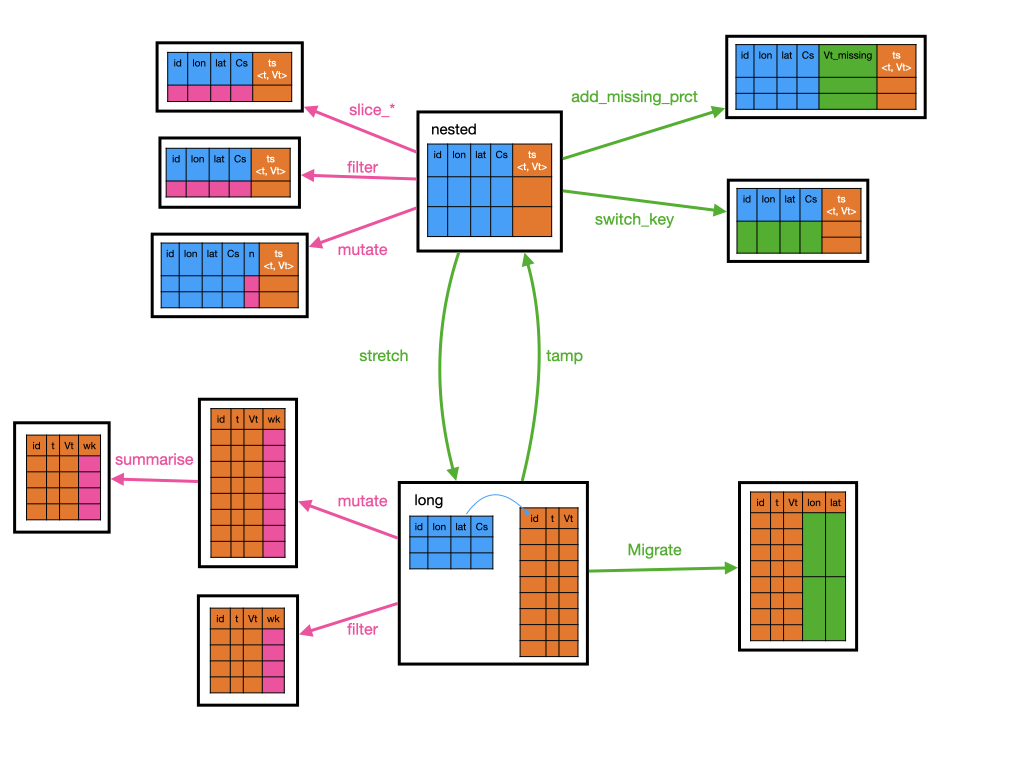
\includegraphics[width=1\linewidth,height=0.5\textheight]{/Users/sherryzhang/Documents/research/paper-cubble/figures/cubble-operations/cubble-operations.001} 

}

\caption{Cubble operations}\label{fig:cubble-operations}
\end{figure}

\hypertarget{basics}{%
\subsubsection{Basics}\label{basics}}

\begin{itemize}
\tightlist
\item
  \texttt{stretch}: nest to long form
\item
  \texttt{tamp}: long to nest form
\item
  \texttt{migrate}: move selected spatial variables to the long form.
\item
  \texttt{add\_dscrb\_prct}: summary stats for missingness
\end{itemize}

dplyr compatibility:

\begin{itemize}
\tightlist
\item
  mutate, filter, summarise, select, arrange
\item
  group and ungroup: group\_by, ungroup
\item
  slice family
\end{itemize}

\hypertarget{combine-two-cubbles}{%
\subsubsection{Combine two cubbles}\label{combine-two-cubbles}}

\begin{itemize}
\tightlist
\item
  match river and weather gauges data
\item
  involve combining two cubbles
\item
  join operations combine the two together by appending more rows but
  what we really want is to bind rows.
\item
  bind rows also doesn't work since we want to bind only when there' s a
  matching????
\item
  introduce bind\_join
\end{itemize}

\hypertarget{hierarchical-structure-in-cubble}{%
\subsubsection{Hierarchical structure in
cubble}\label{hierarchical-structure-in-cubble}}

\begin{itemize}
\tightlist
\item
  hierarchical is common.
\item
  Given examples.
\item
  Essence: switch between different levels
\item
  introduce \texttt{switch\_key}
\end{itemize}

\newpage

\hypertarget{examples}{%
\section{Examples}\label{examples}}

Daily climate data (prcp, tmax, and tmin) from RNOAA - lots of stations
across Australia

An exploratory data analysis questions: What's the climate profile look
like in Australia

\begin{itemize}
\tightlist
\item
  General features: Any general trend/ fluctuation in prcp, tmax, and
  tmin?
\item
  Local features: Any station stands out from the crowd?
\end{itemize}

\hypertarget{manipulation}{%
\subsection{Manipulation}\label{manipulation}}

\hypertarget{mutate-and-filter}{%
\subsubsection{Mutate and filter}\label{mutate-and-filter}}

In the first example, we want to only keep the stations that have
\texttt{tmax} recorded in 2020. This requires first narrow down the
records to those in 2020, determine if \texttt{tmax} is missing for each
station, and then retain those stations that have \texttt{tmax}
recorded. The year filtering is an operation on the time axis, so we
start with the long form. Whether each station has \texttt{tmax}
recorded is a result of each station, rather than of each time point,
hence we need to switch to the nested form with \texttt{tamp()}. To
calculate whether \texttt{tmax} is recorded, we mutate a column
\texttt{tmax\_missing} that takes \texttt{TRUE} if all the \texttt{tmax}
in the nested list column \texttt{ts} are \texttt{NA} and \texttt{FALSE}
otherwise. To get the stations that we want, we need another filter on
\texttt{tmax\_missing}.

\begin{Shaded}
\begin{Highlighting}[]
\NormalTok{aus\_climate }\SpecialCharTok{\%\textgreater{}\%} 
  \FunctionTok{stretch}\NormalTok{() }\SpecialCharTok{\%\textgreater{}\%} 
  \FunctionTok{filter}\NormalTok{(}\FunctionTok{year}\NormalTok{(date) }\SpecialCharTok{==} \DecValTok{2020}\NormalTok{) }\SpecialCharTok{\%\textgreater{}\%} 
  \FunctionTok{tamp}\NormalTok{()}
\end{Highlighting}
\end{Shaded}

\begin{verbatim}
## # Cubble: id-wise: nested form
## # Key:    id [85]
## # Leaves: date [date], prcp [dbl], tmax [dbl], tmin [dbl]
##    id            lat  long  elev name                   wmo_id ts               
##    <chr>       <dbl> <dbl> <dbl> <chr>                   <dbl> <list>           
##  1 ASN00009021 -31.9  116.  15.4 perth airport           94610 <tibble [366 x 4~
##  2 ASN00010311 -31.9  117. 179   york                    94623 <tibble [366 x 4~
##  3 ASN00010614 -32.9  117. 338   narrogin                94627 <tibble [366 x 4~
##  4 ASN00014015 -12.4  131.  30.4 darwin airport          94120 <tibble [366 x 4~
##  5 ASN00015131 -17.6  134. 220   elliott                 94236 <tibble [366 x 4~
##  6 ASN00016065 -30.4  137.  76   andamooka               95660 <tibble [366 x 4~
##  7 ASN00023034 -35.0  139.   2   adelaide airport        94672 <tibble [366 x 4~
##  8 ASN00023373 -34.5  139. 275   nuriootpa viticultural  94681 <tibble [366 x 4~
##  9 ASN00024024 -34.4  141.  30.1 loxton research centre  94682 <tibble [366 x 4~
## 10 ASN00024048 -34.2  141.  31.5 renmark aero            95687 <tibble [366 x 4~
## # ... with 75 more rows
\end{verbatim}

\hypertarget{join}{%
\subsubsection{Join}\label{join}}

Now we want to select the stations that have been registered with world
meteorological organisation (WMO) and the dataset \texttt{station} has a
column \texttt{wmo\_id} that records this information. To do this task,
we first need to join the \texttt{station} dataset with our climate
dataset and then filter out those stations that don't have the WMO id.
Since the join is by station rather than by time, we start with the
nested form and write the exact same syntax of join and filter as with
tidyverse.

\begin{Shaded}
\begin{Highlighting}[]
\CommentTok{\# join wmo\_id for each station}
\CommentTok{\# to\_join \textless{}{-} station \%\textgreater{}\% select(id, wmo\_id)}
\CommentTok{\# out \textless{}{-} climate\_small \%\textgreater{}\% }
\CommentTok{\#   left\_join(to\_join, by = c("station" = "id")) \%\textgreater{}\% }
\CommentTok{\#   filter(!is.na(wmo\_id))}
\CommentTok{\# out}
\end{Highlighting}
\end{Shaded}

Sometimes, we would like to have station-wise and time-wise variables in
the same form (i.e.~when plotting glyph maps). This can also be seen as
a joining task, on the long form, with the dataset to join being the
metadata. \texttt{migrate()} is a verb introduced as the shortcut for
\texttt{left\_join()} with a cubble's metadata and below is the
comparison of the two syntaxes.

\begin{Shaded}
\begin{Highlighting}[]
\NormalTok{aus\_climate }\SpecialCharTok{\%\textgreater{}\%} 
  \FunctionTok{stretch}\NormalTok{() }\SpecialCharTok{\%\textgreater{}\%} 
  \FunctionTok{migrate}\NormalTok{(id, lat, long)}
\end{Highlighting}
\end{Shaded}

\begin{verbatim}
## # Cubble: time-wise: long form
## # Key:    id [85]
## # Leaves: id [chr], lat [dbl], long [dbl], elev [dbl], name [chr], wmo_id
## #   [dbl], prcp_missing [dbl], tmax_missing [dbl], tmin_missing [dbl]
##    id          date        prcp  tmax  tmin   lat  long
##    <chr>       <date>     <dbl> <dbl> <dbl> <dbl> <dbl>
##  1 ASN00009021 2020-01-01     0   319   153 -31.9  116.
##  2 ASN00009021 2020-01-02     0   249   164 -31.9  116.
##  3 ASN00009021 2020-01-03     6   232   130 -31.9  116.
##  4 ASN00009021 2020-01-04     0   284   124 -31.9  116.
##  5 ASN00009021 2020-01-05     0   353   116 -31.9  116.
##  6 ASN00009021 2020-01-06     0   348   131 -31.9  116.
##  7 ASN00009021 2020-01-07     0   328   151 -31.9  116.
##  8 ASN00009021 2020-01-08     0   304   174 -31.9  116.
##  9 ASN00009021 2020-01-09     0   287   173 -31.9  116.
## 10 ASN00009021 2020-01-10     0   326   158 -31.9  116.
## # ... with 31,100 more rows
\end{verbatim}

\begin{itemize}
\tightlist
\item
  data quality check: filter out stations have variables not properly
  recorded
\item
  data summary:

  \begin{itemize}
  \tightlist
  \item
    daily -\textgreater{} monthly/ weekly,
  \item
    summarise by mean for tmax/ tmin, sum for prcp
  \end{itemize}
\item
\end{itemize}

\hypertarget{graphics}{%
\subsection{Graphics}\label{graphics}}

Static + interactive -\textgreater{} tooltip to show additional
information upon hovering

\begin{itemize}
\tightlist
\item
  Where are those stations on the map?

  \begin{itemize}
  \tightlist
  \item
    Mention mostly aero, airport, and lighthouse
  \end{itemize}
\end{itemize}

\hypertarget{summary}{%
\section*{Summary}\label{summary}}
\addcontentsline{toc}{section}{Summary}

\hypertarget{refs}{}
\begin{CSLReferences}{1}{0}
\leavevmode\hypertarget{ref-stars}{}%
Pebesma, Edzer. 2021. \emph{Stars: Spatiotemporal Arrays, Raster and
Vector Data Cubes}. \url{https://CRAN.R-project.org/package=stars}.

\leavevmode\hypertarget{ref-pebesma2018simple}{}%
Pebesma, Edzer J. 2018. {``Simple Features for r: Standardized Support
for Spatial Vector Data.''} \emph{R J.} 10 (1): 439.

\leavevmode\hypertarget{ref-tsibbles}{}%
Wang, Earo, Dianne Cook, and Rob J Hyndman. 2020. {``A New Tidy Data
Structure to Support Exploration and Modeling of Temporal Data.''}
\emph{Journal of Computational and Graphical Statistics} 29 (3):
466--78. \url{https://doi.org/10.1080/10618600.2019.1695624}.

\end{CSLReferences}

\bibliographystyle{unsrt}
\bibliography{references.bib}


\end{document}
